\documentclass[11pt, a4paper]{article}

\usepackage{amsmath, amssymb, titling}
\usepackage[margin=2.5cm]{geometry}
\usepackage[colorlinks=true, linkcolor=black, urlcolor=black, citecolor=black]{hyperref}
\usepackage{graphicx}
\usepackage{float}
\usepackage{cancel}
\usepackage{fancyhdr, lastpage}
\usepackage{fourier-orns}
\usepackage{xcolor}

% \usepackage{minted}

\renewcommand\maketitlehooka{\null\mbox{}\vfill}
\renewcommand\maketitlehookd{\vfill\null}
\renewcommand{\headrule}{
\vspace{-5pt}\hrulefill
\raisebox{-2.1pt}{\quad\leafleft\decoone\leafright\quad}\hrulefill}

\title{Dynamics and Stability of Multiphase Flows \\ HW4}
\author{Almog Dobrescu\\\\ID 214254252}

\pagestyle{fancy}
\cfoot{Page \thepage\ of \pageref{LastPage}}

\begin{document}

\maketitle

\thispagestyle{empty}
\newpage
\setcounter{page}{1}

\tableofcontents
\vfil
\listoffigures
\newpage

\section{Velocity Profile $U_{\left(z\right)}$ as a Funciton of \emph{z}}
Consider a liquid jet ejected from a circular orifice of radius \emph{a} (point A). The jet has flux \emph{Q} of fluid with density $\rho$ that exits with velocity $U_0$. The surface tension between the fluid and the air with pressure $P_0$ is $\sigma$. \\
By assuming laminar, inviscid, incpmressible, axisymmetric and steady flow, we get the Bernoulli equation, between point A and arbitrary point downstream B:
\begin{equation}
    \frac{1}{2}\rho U_0^2+\rho gz+P_A=\frac{1}{2}\rho U_{\left(z\right)}^2+P_B
\end{equation}
The Laplace pressure for a jet:
\begin{equation}
    \begin{array}{c}
        \begin{matrix}
            \displaystyle\Delta P=\sigma\left(\frac{1}{R_1}+\frac{1}{R_2}\right) && \left\{\begin{array}{l}
                R_1=R_{1\left(z\right)}=\text{inner radius (normal to the flow)} \\
                R_2=R_{2\left(z\right)}=\text{outer radius (parallel to the flow)}
            \end{array}\right.
        \end{matrix} \\\\
        \Downarrow \\
        \begin{matrix}
            \displaystyle P_A=P_0+\sigma\left(\frac{1}{a}\right) && \displaystyle P_B=P_0+\sigma\left(\frac{1}{R_1}+\frac{1}{R_2}\right)
        \end{matrix}
    \end{array}
\end{equation}
substituting into the Bernoulli equation:
\begin{equation}
    \frac{1}{2}\rho U_0^2+\rho gz+\cancel{P_0}+\frac{\sigma}{a}=\frac{1}{2}\rho U_{\left(z\right)}^2+\cancel{P_0}+\sigma\left(\frac{1}{R_1}+\frac{1}{R_2}\right)
\end{equation}
Isolating $U_{\left(z\right)}$ we get:
\begin{equation}
    \frac{U_{\left(z\right)}}{U_0}=\sqrt{1+\frac{2gz}{U_0^2}+\frac{2\sigma}{\rho U_0^2}\left(\frac{1}{a}-\frac{1}{R_1}-\frac{1}{R_2}\right)}
\end{equation}
and in dimensionless form:
\begin{equation}
    \frac{U_{\left(z\right)}}{U_0}=\sqrt{1+\underbrace{\frac{2z}{Fr^2a}}_{\substack{\text{acceleration}\\\text{due to gravity}}}+\underbrace{\frac{2}{We}\left(1-\frac{a}{R_1}-\frac{a}{R_2}\right)}_{\substack{\text{deceleration}\\\text{due to surface tension}}}}
\end{equation}
where:
\begin{itemize}
    \item $\displaystyle We=\frac{\rho U_0^2a}{\sigma}$ is the Webber \#
    \item $\displaystyle Fr=\frac{U_0^2}{ga}$ is the Froud \#
\end{itemize}
Let's consider the curvature of the wall of the get parallel to the flow:
\begin{equation}
    \underbrace{\kappa}_{\substack{\text{principal}\\\text{curvature}}}=-\frac{R_{1zz}}{\left(1+R_{1z}^2\right)^{\frac{3}{2}}}\underbrace{=}_{\text{linearization}}-R_{1zz}
\end{equation}
The principal curvature equals one over the principal radius so:
\begin{equation}
    \kappa=\frac{1}{R_2}=-\frac{\partial^2 R_1}{\partial z^2}
\end{equation}
So, the velocity profile $U_{\left(z\right)}$ as a funciton of \emph{z} is therefore:
\begin{equation}
    \colorbox{yellow}{$\displaystyle\frac{U_{\left(z\right)}}{U_0}=\sqrt{1+\frac{2z}{Fr^2a}+\frac{2}{We}\left(1-\frac{a}{R_1}+a\frac{\partial^2 R_1}{\partial z^2}\right)}$}
\end{equation}

\newpage

\section{ODE of Jet Radius $r_{\left(z\right)}$}
\subsection{Formulate the ODE}
From conservation of flux:
\begin{equation}
    \begin{array}{c}
        \displaystyle Q=2\pi\int_0^{R_1}U_{\left(z\right)}rdr=\pi R_1^2U_{\left(z\right)}\underbrace{=}_{z=0}\pi a^2U_0 \\\\
        Q_{\left(z\right)}=\pi U_{\left(z\right)}R_1^2\underbrace{=}_{\substack{\text{conservation}\\\text{of mass}}}\pi a^2U_0 \\\\
        \Downarrow \\
        \displaystyle \frac{R_1}{a}=\sqrt{\frac{U_0}{U_{\left(z\right)}}}
    \end{array}
\end{equation}
After substituting $U_{\left(z\right)}$:
\begin{equation}
    \colorbox{yellow}{$\displaystyle R_1=\frac{a^2U_0}{\displaystyle\sqrt{U_0^2+2gz+\frac{2\sigma}{\rho}\left(\frac{1}{a}-\frac{1}{R_1}+\frac{\partial^2 R_1}{\partial z^2}\right)}}$}
\end{equation}

\subsection{Boundary Conditions}
Assume BC:
\begin{enumerate}
    \item $R_{1\left(z=0\right)}=a$
    \item $\displaystyle\left.\frac{\partial R_1}{\partial z}\right|_{z=0}=0$
\end{enumerate}
The first conditions is given. \\
The second condition is derived from the fact that at the begining, the jet looks like a cylinder.
\newpage

\section{Numerical Solver}
The selected method is the Runge-Kutta-Merson method. \\
Isolating the second derivitive of $R_1$:
\begin{equation}
    \begin{array}{rcl}
        \displaystyle\frac{a^4}{R_1^4}&=&\displaystyle1+\frac{2z}{\text{Fr}^2a}+\frac{2}{\text{We}}\left(1-\frac{a}{R_1}+a\frac{\partial^2 R_1}{\partial z^2}\right) \\\\
        \displaystyle\frac{\text{We}\cdot a^4}{2R_1^4}&=&\displaystyle\frac{\text{We}}{2}+\frac{\text{We}z}{\text{Fr}^2a}+1-\frac{a}{R_1}+a\frac{\partial^2R_1}{\partial z^2} \\\\
        \displaystyle\frac{\partial^2R_1}{\partial z^2}&=&\displaystyle\frac{\text{We}\cdot a^3}{2R_1^4}-\frac{\text{We}}{2a}-\frac{\text{We}\cdot z}{\text{Fr}^2a^2}-\frac{1}{a}+\frac{1}{R_1}
    \end{array}
\end{equation}
% Where:
% \begin{equation}
%     \begin{array}{rcl}
%         \displaystyle\left.\frac{\partial^2R_1}{\partial z^2}\right|_i=\displaystyle f^{''}_i&=&\displaystyle\frac{\delta^2f_i}{h^2} \\\\
%         &=&\displaystyle\frac{\delta\left(f_{i+\frac{1}{2}}-f_{i-\frac{1}{2}}\right)}{h^2} \\\\
%         &=&\displaystyle\frac{\left(f_{i+1}-2f_{i}+f_{i-1}\right)}{h^2}
%     \end{array}
% \end{equation}
% So the ODE becomes:
% \begin{equation}
%     R_{1,i+1}=\left(\displaystyle\frac{\text{We}\cdot a^3}{2R_1^4}-\frac{\text{We}}{2a}-\frac{\text{We}z}{\text{Fr}^2a^2}-\frac{1}{a}+\frac{1}{R_1}\right)h^2+2R_{1,i}-R_{1,i-1}
% \end{equation}
Defining the system of equations:
\begin{equation}
    \begin{matrix}
        x=R_1 &&& y=\displaystyle\frac{\partial R_1}{\partial z}
    \end{matrix}
\end{equation}
\begin{equation}
    \begin{matrix}
        \left\{\begin{array}{rcl}
            \displaystyle\frac{\partial x}{\partial z}&=&g_{\left(z,x,y\right)} \\\\
            \displaystyle\frac{\partial y}{\partial z}&=&f_{\left(z,x,y\right)}
        \end{array}\right. &\text{where}& \begin{array}{rcl}
            g&=&y \\\\
            f&=&\displaystyle\frac{\text{We}\cdot a^3}{2x^4}-\frac{\text{We}}{2a}-\frac{\text{We}\cdot z}{\text{Fr}^2a^2}-\frac{1}{a}+\frac{1}{x}
        \end{array}
    \end{matrix}
\end{equation}
The Runge-Kutta-Merson method is defined as:
\begin{equation}
    \begin{array}{l}
        \left\{\begin{array}{rcl}
            x_{i+1}&=&\displaystyle x_i+\frac{1}{6}\left(m_1+4m_4+m_5\right) \\\\
            y_{i+1}&=&\displaystyle y_i+\frac{1}{6}\left(k_1+4k_4+k_5\right)
        \end{array}\right. \\\\
        \left\{\begin{array}{rcl}
            m_1&=&hg_{\left(z_i, x_i, y_i\right)} \\
            k_1&=&hf_{\left(z_i, x_i, y_i\right)}
        \end{array}\right. \\\\
        \left\{\begin{array}{rcl}
            m_2&=&hg_{\left(z_i+\frac{1}{3}h, x_i+\frac{1}{3}m_1, y_i+\frac{1}{3}k_1\right)} \\
            k_2&=&hf_{\left(z_i+\frac{1}{3}h, x_i+\frac{1}{3}m_1, y_i+\frac{1}{3}k_1\right)}
        \end{array}\right. \\\\
        \left\{\begin{array}{rcl}
            m_3&=&hg_{\left(z_i+\frac{1}{3}h, x_i+\frac{1}{6}\left(m_1+m_2\right), y_i+\frac{1}{6}\left(k_1+k_2\right)\right)} \\
            k_3&=&hf_{\left(z_i+\frac{1}{3}h, x_i+\frac{1}{6}\left(m_1+m_2\right), y_i+\frac{1}{6}\left(k_1+k_2\right)\right)} 
        \end{array}\right. \\\\
        \left\{\begin{array}{rcl}
            m_4&=&hg_{\left(z_i+\frac{1}{2}h, x_i+\frac{1}{8}\left(m_1+3m_3\right), y_i+\frac{1}{8}\left(k_1+3k_3\right)\right)} \\
            k_4&=&hf_{\left(z_i+\frac{1}{2}h, x_i+\frac{1}{8}\left(m_1+3m_3\right), y_i+\frac{1}{8}\left(k_1+3k_3\right)\right)} 
        \end{array}\right. \\\\
        \left\{\begin{array}{rcl}
            m_5&=&hg_{\left(z_i+h, x_i+\frac{1}{2}\left(m_1-3m_3+4m_4\right), y_i+\frac{1}{2}\left(k_1-3k_3+4k_4\right)\right)} \\ 
            k_5&=&hf_{\left(z_i+h, x_i+\frac{1}{2}\left(m_1-3m_3+4m_4\right), y_i+\frac{1}{2}\left(k_1-3k_3+4k_4\right)\right)} 
        \end{array}\right.
    \end{array}
\end{equation}

\newpage

\section{Solution}
\begin{equation}
    \begin{matrix}
        \displaystyle U_0=1\left[\frac{\mathrm{m}}{\mathrm{sec}}\right] & a=0.05\left[\mathrm{m}\right] & \displaystyle\rho=998\left[\frac{\mathrm{kg}}{\mathrm{m}^3}\right] & \displaystyle\sigma=0.0728\left[\frac{\mathrm{N}}{\mathrm{m}}\right] & \displaystyle g=9.81\left[\frac{\mathrm{m}}{\mathrm{sec}^2}\right] \\\\
        & h=10^{-5}\left[m\right] && z=\left[0,h,2h,\cdots,5\right]\left[m\right]
    \end{matrix}
\end{equation}
\begin{figure}[H]
    \centering
    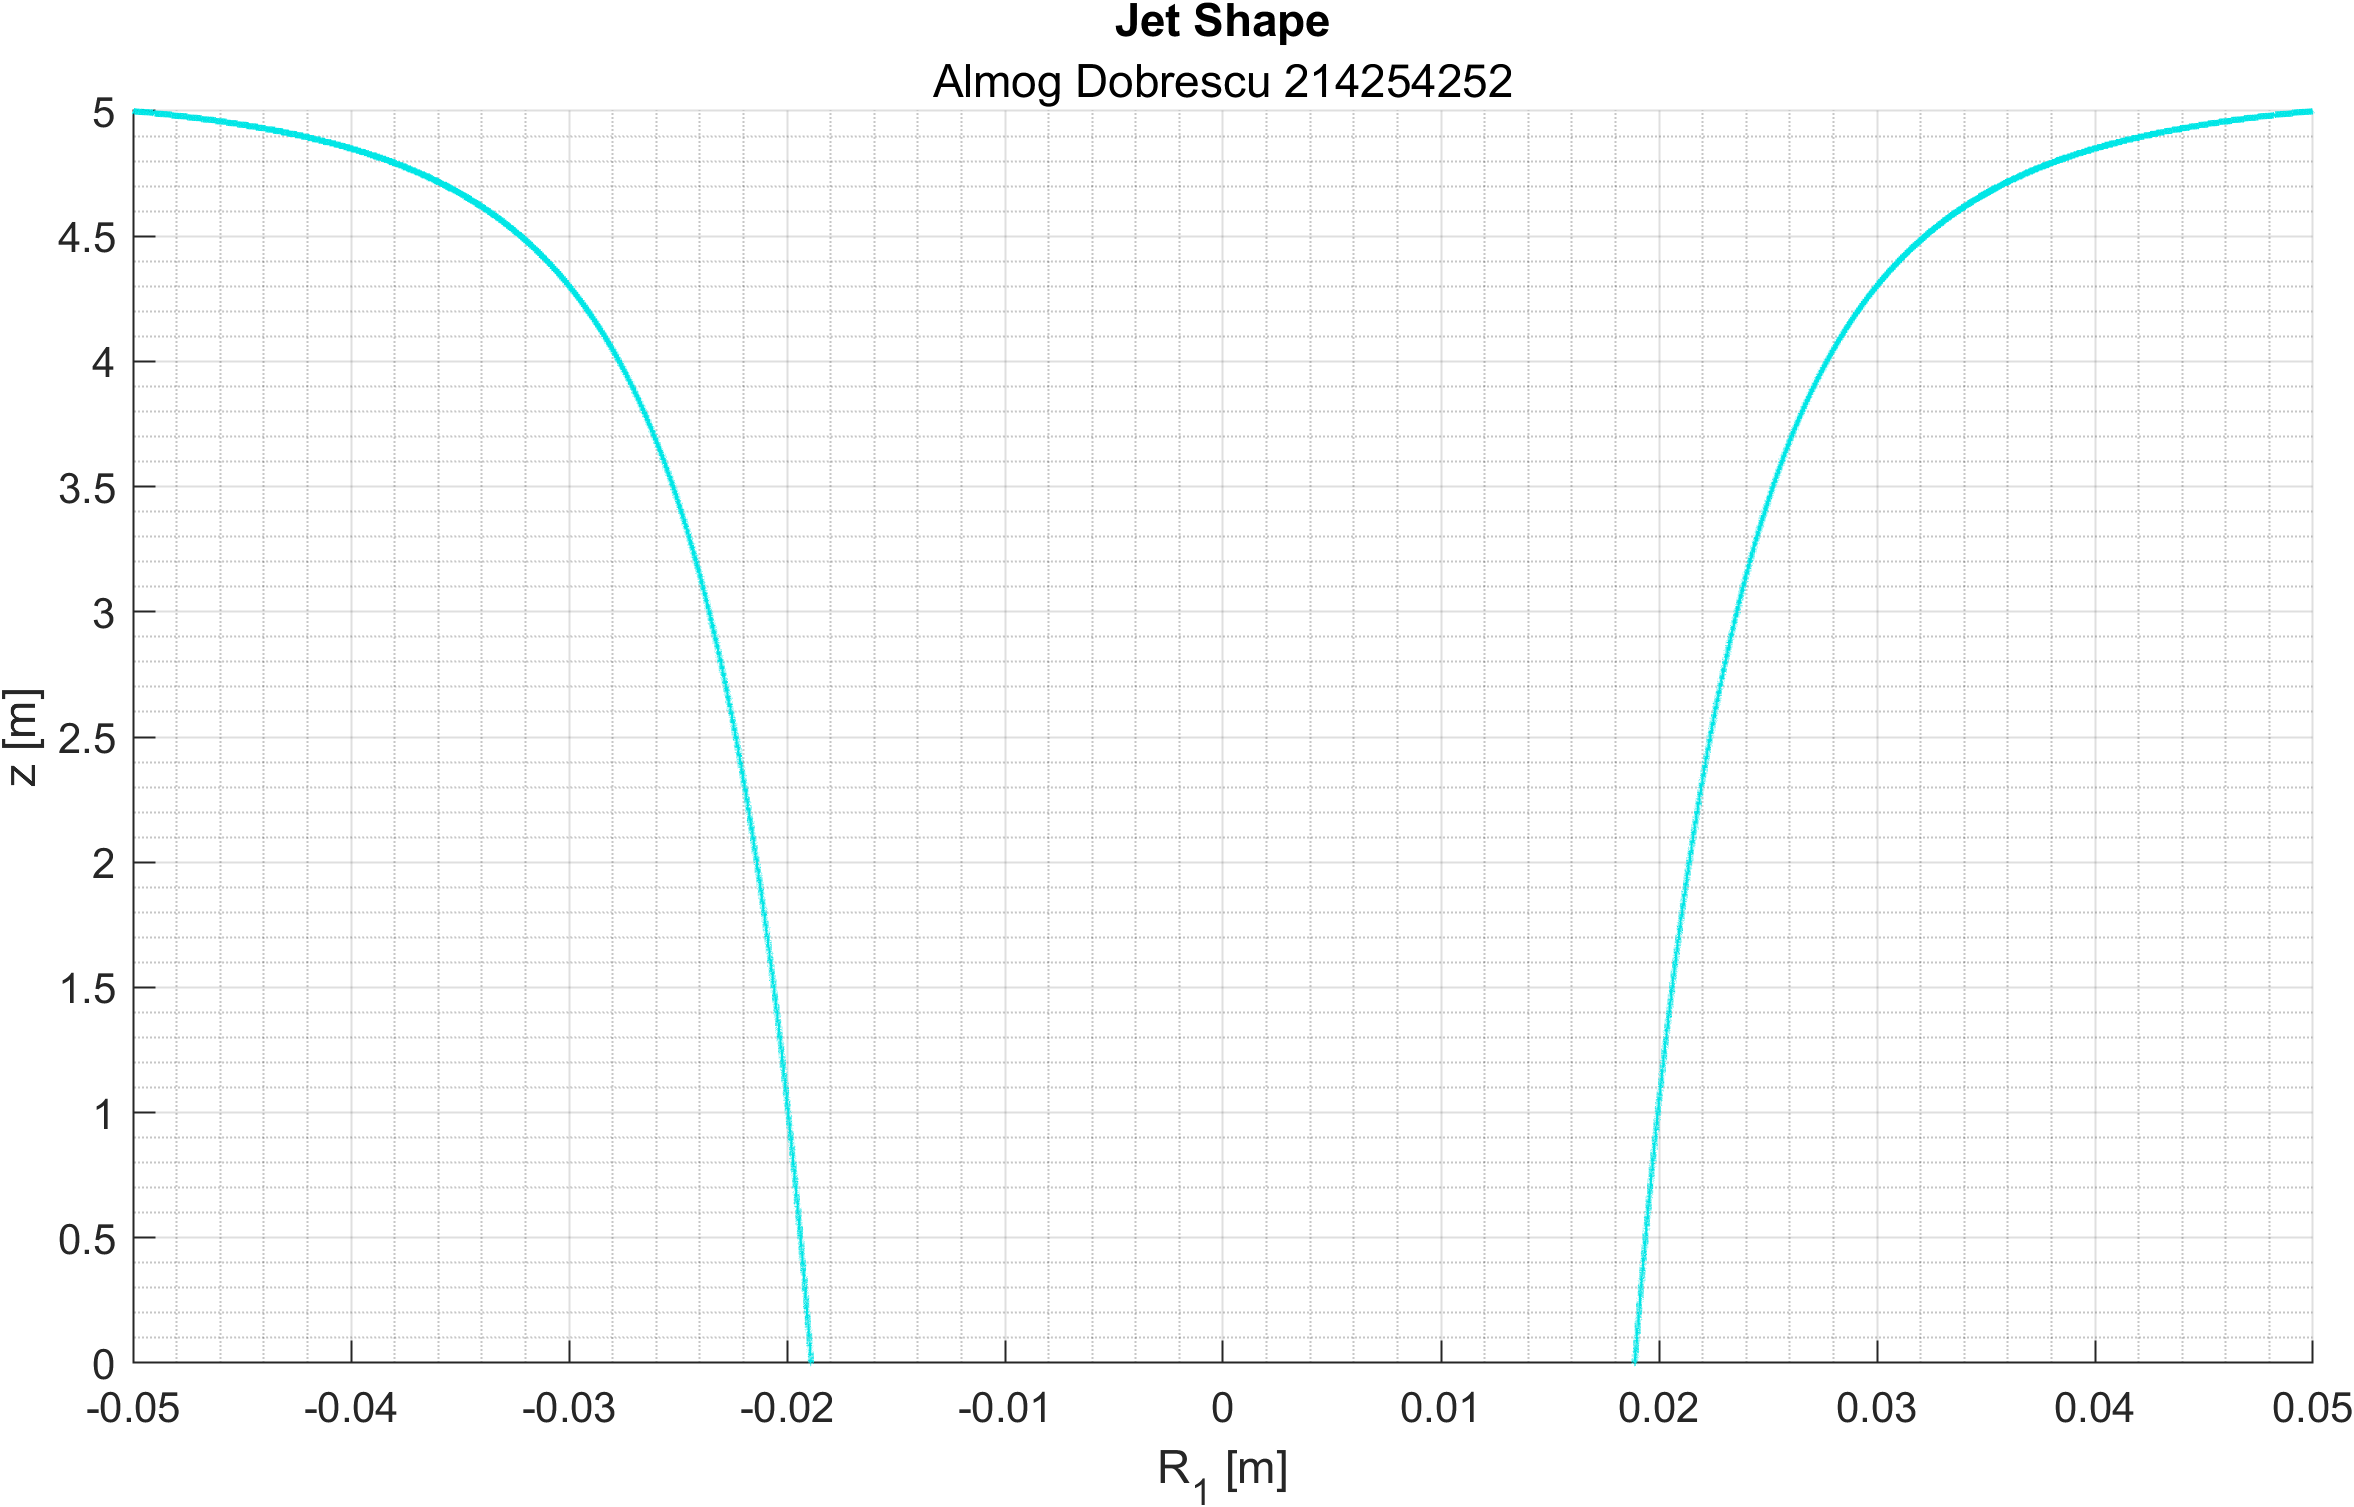
\includegraphics[width=0.85\textwidth]{images/graph1.png}
    \caption{The jet shape}
    \label{fig:The_jet_shape}
\end{figure}
\begin{figure}[H]
    \centering
    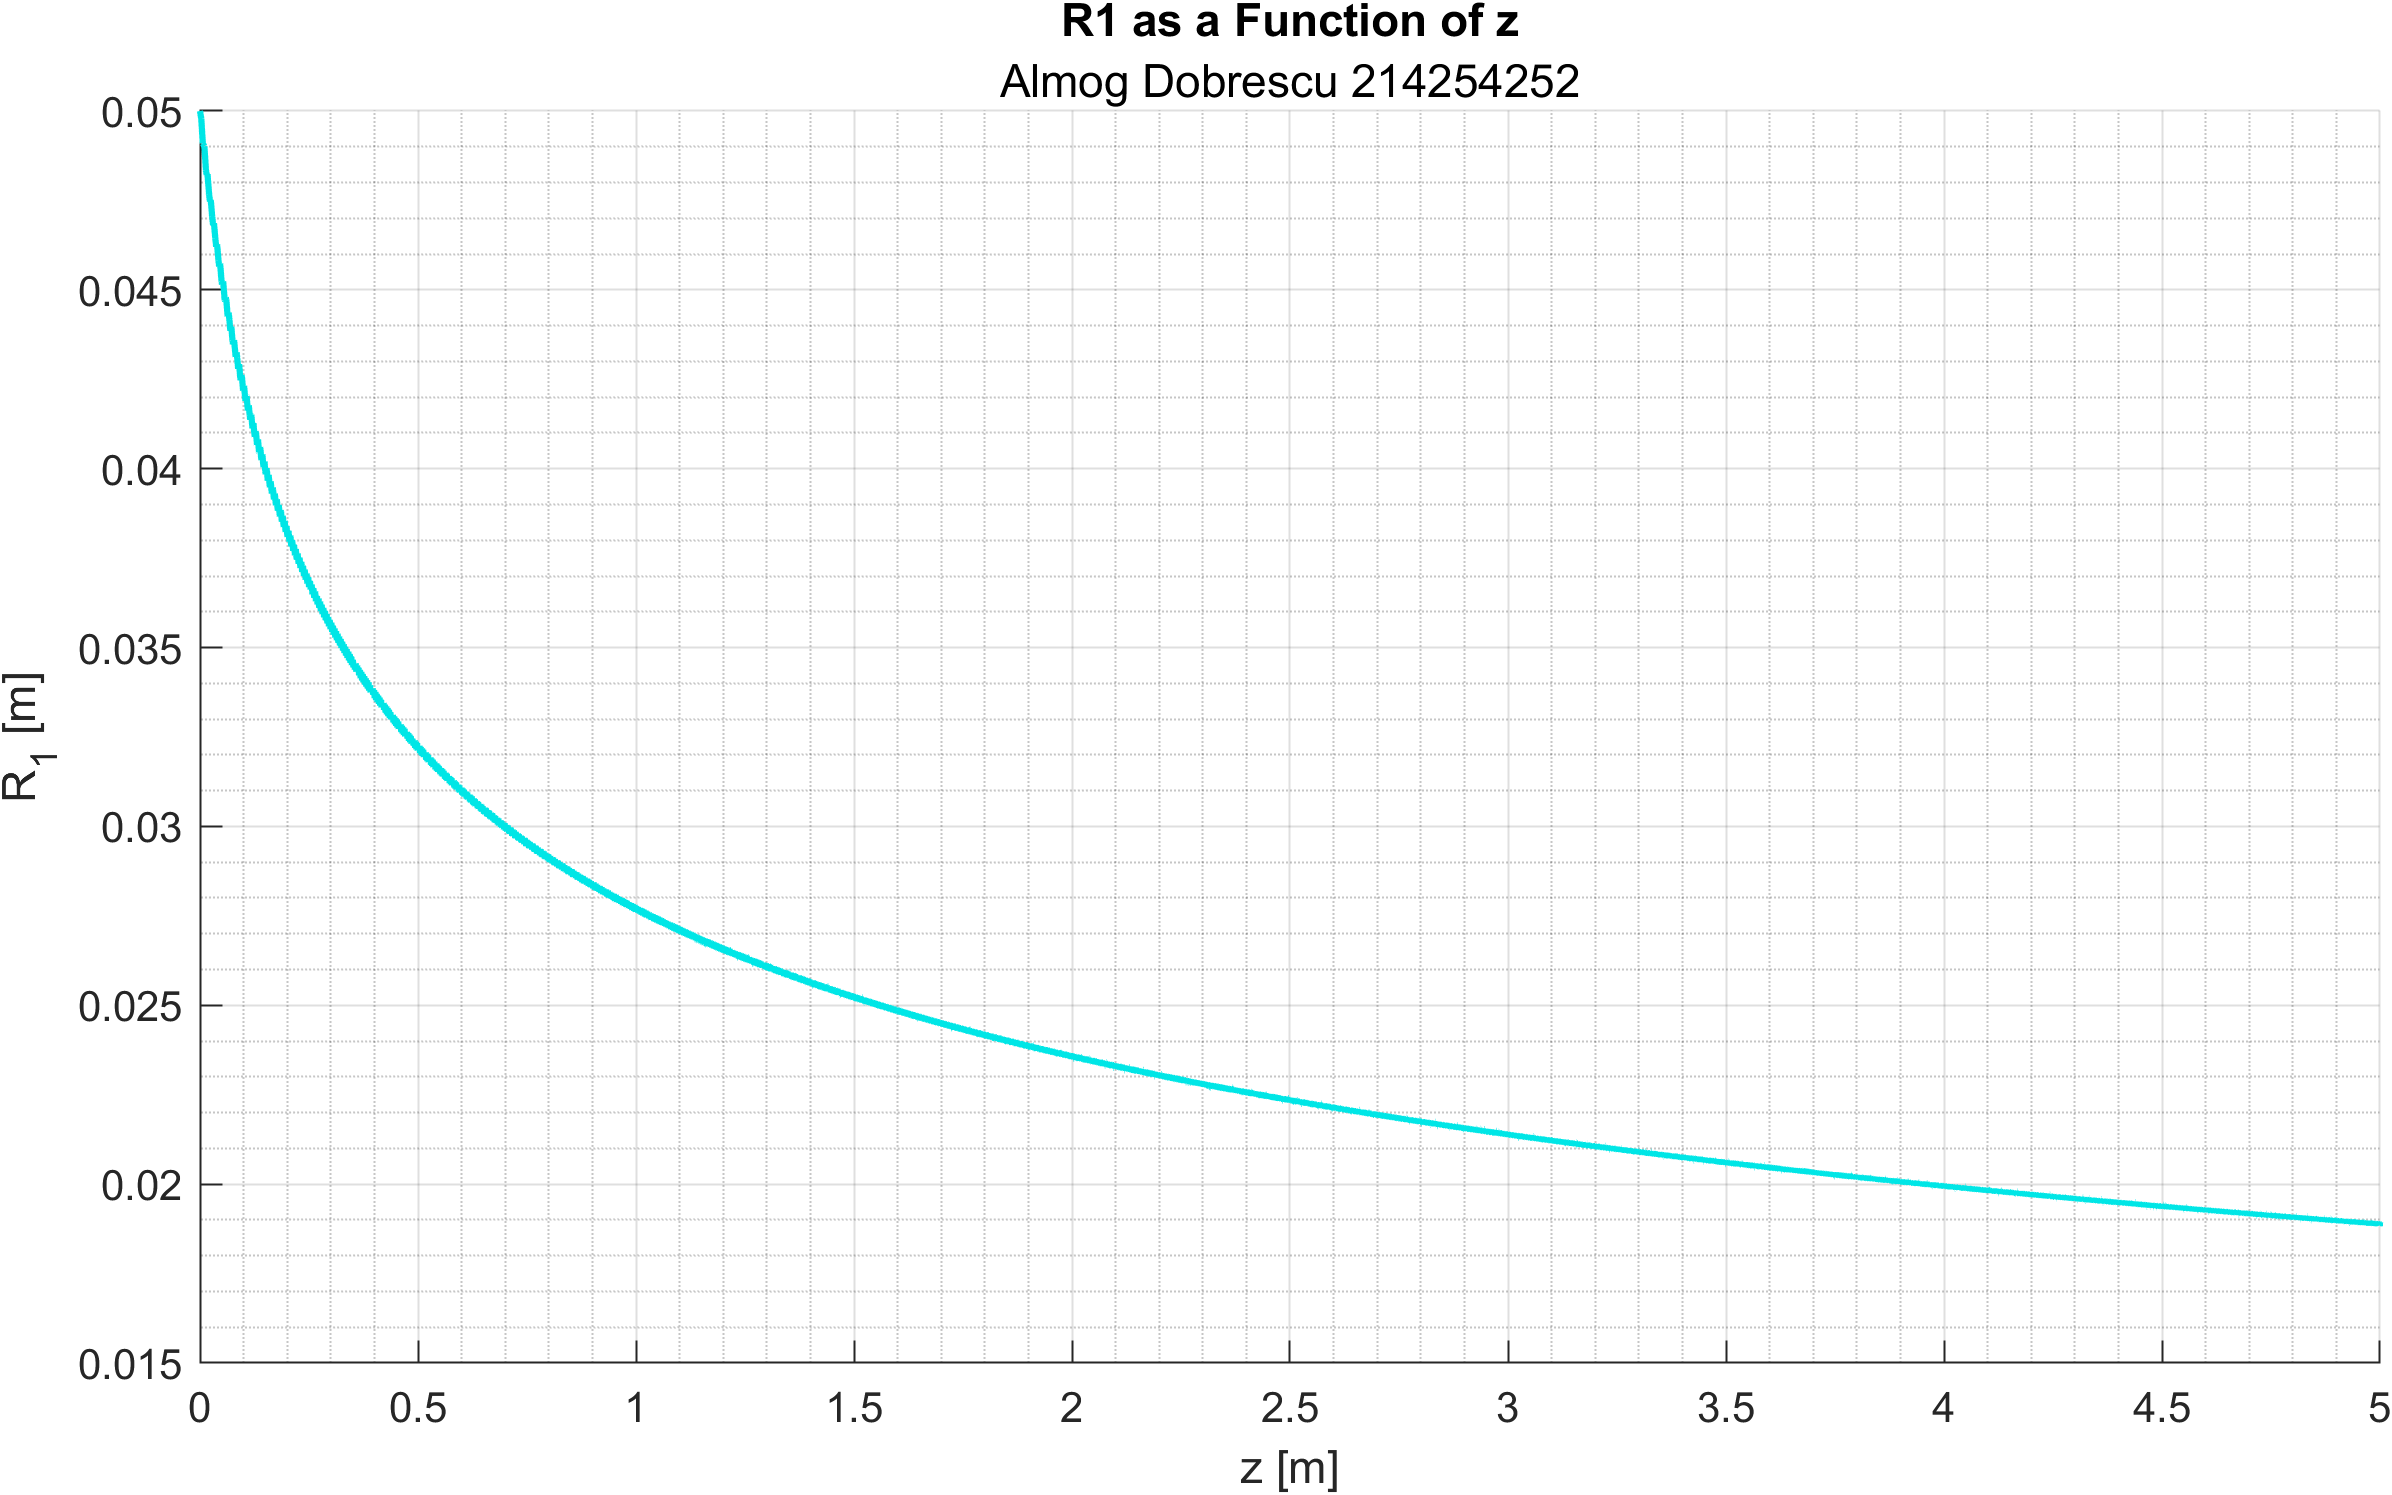
\includegraphics[width=0.85\textwidth]{images/graph2.png}
    \caption{$R_1$ as a function of z}
    \label{fig:R_1_of_z}
\end{figure}

\section{Compering The Results}


\end{document}